\begin{quote}
	\textit{``If the chaos of the nineties reflects a radical shift in the paradigms of visual literacy, the final shift away from the Lascaux/Gutenberg tradition of a pre-holographic society, what should we expect from this newer technology, with his promise of discrete encoding and subsequent reconstruction of the full range of sensory perception?''}
\end{quote}
\hfill \textit{Burning Chrome, William Gibson}
\\
\\

%=========================================================================================================

\label{chapter-conclusions}

Alternate realities have fascinated mankind since early prehistory and with the advent of the computer and the smartphone we have seen the rise of many different categories of alternate reality that replace, augment, diminish and mix with our familiar real world to expand our capabilities and our understanding. This thesis has introduced parallel reality as a new category of alternate reality that comprises two environments, one real and the other virtual, each complete unto itself and wherein the user may freely switch between them. The benefits that such a system imparts upon the user by granting them the ability to mitigate the vacancy problem and explore parallel real and virtual environments in tandem has been shown through the development of the Mirrorshades parallel reality platform and its application to a use case within the realm of cultural heritage. Evaluation of these studies has lead to the establishment of a number of best practices for future parallel reality endeavours.

\begin{figure}[t]
	\begin{center}
		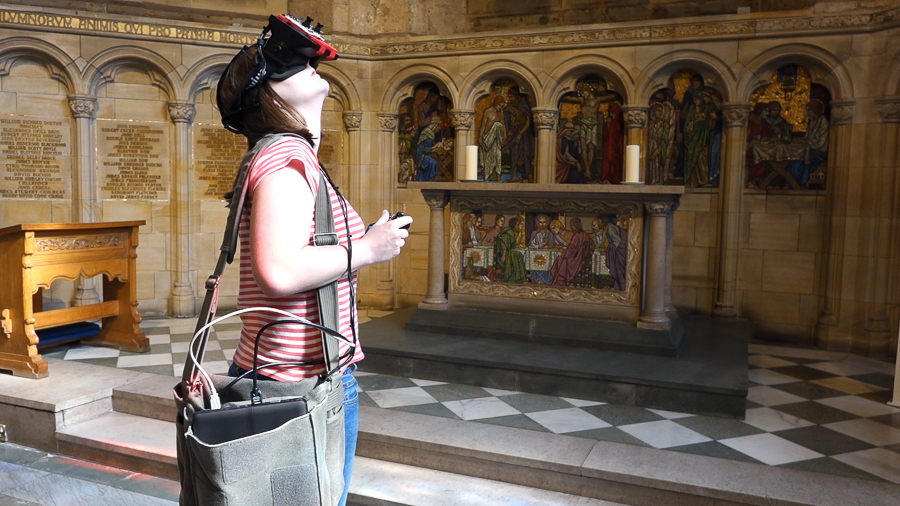
\includegraphics[width=\textwidth]{participant-f-4.jpg}
		\caption{The Mirrorshades parallel reality platform in use at a 15th century chapel.}
		\label{participant-f-4.jpg}
	\end{center}	
\end{figure}

\begin{figure}[t]
	\begin{center}
		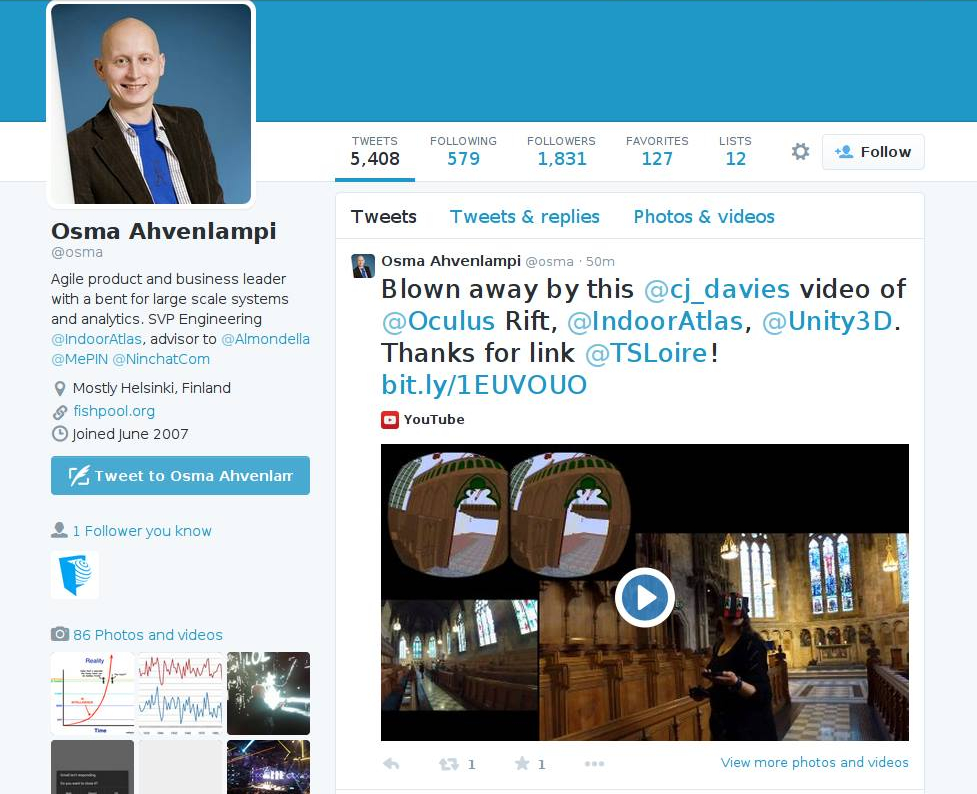
\includegraphics[width=0.8\textwidth]{osma-twitter.jpg}
		\caption{Praise for the Mirrorshades parallel reality platform from IndoorAtlas' senior vice president of engineering.}
		\label{osma-twitter.jpg}
	\end{center}	
\end{figure}

%=========================================================================================================

\section{Contributions}

As listed in section \ref{intro-contributions} the contributions of this thesis can be summarized as follows:

\begin{itemize}
	\item The introduction of parallel reality as a new category of alternate reality that allows users to experience complete real and virtual environments in tandem and represents an avenue for further mitigation of the vacancy problem.
	\item The framing of parallel reality through a thorough investigation and extension of previous taxonomies that classify and distinguish between alternate reality terminologies.
	\item The presentation of the combined Milgram/Waterworth model for visualising alternate reality experiences, including those of parallel reality systems.
	\item Development of a preliminary parallel reality platform, the Virtual Time Window, through extension of the Second Life client.
	\item Development of a second parallel reality platform, dubbed Mirrorshades, that combines new virtual reality hardware with novel indoor positioning technology.
	\item Evaluation of the Mirrorshades platform through user studies of a real world use case study within the realm of virtual heritage, including the discussion and application of an established presence questionnaire to a parallel reality experience.
	\item Creation and discussion of a set of best practices for future parallel reality endeavours.
\end{itemize}

%=========================================================================================================

\section{Future Work}

The introduction of parallel reality in this thesis along with the investigation of its first involved implementations in the VTW and Mirrorshades platforms is only the beginning of en extended course of study that will be required to fully understand and come to appreciate the benefits that it can provide as a concept. The following discussion highlights but a few choice avenues that the investigation into parallel reality would do well to explore and should by no means be considered an exhaustive list of possible sources of extension; after all the \textit{``potential applications of VR are really only limited by the imaginations of talented individuals''}~\cite{Giuseppe2014a}. Since its recent rejuvenation at the hands of Oculus, the field of virtual reality has seen its rate of progress and advancement massively accelerated. With this in mind, the potential of these avenues of further investigation into the parallel reality concept to produce fruitful research is substantial.

Most evident is the matter of hardware. The Mirrorshades parallel reality platform used in the case study presented in this thesis is a somewhat cumbersome package of HMD, laptop, battery pack, smartphone, games console controller and myriad cables, occupying both of the user's hands and requiring them to carry a satchel of not insubstantial size and weight. To posit that the cumbersome nature of the platform had a directly detrimental effect upon the quality of experience received by the participants is no stretch of the imagination and improvements in this regard will be required for parallel reality to see deployment and use in anything but controlled laboratory or user study conditions. As discussed in section \ref{mobile-client} we are already beginning to see the advent of hardware platforms that present a much improved basis for parallel reality experiences. A platform such as Samsung Gear VR, perhaps modified with stereo video see-through abilities, would represent a fully contained single unit parallel reality experience, suitable for handing to a user in the same manner that audio guides are given out at many of the world's museums. Google's Cardboard platform\footnote{\url{https://www.google.com/get/cardboard/}} also presents an intriguing possibility for future parallel reality implementations at very low cost, making use of nothing more than a folded piece of cardboard and two plastic lenses combined with any of a wide variety of smartphones to form a rudimentary HMD which users could bring to their eyes to perform a transition into VR and remove when they wish to view their real surroundings again. Furthermore, improvements to the performance of the platforms, in terms of the visual acuity of both real and virtual content as well as the accuracy of the positioning and registration, will present beneficial results both to casual users and to experts wishing to use such a modality of interaction for serious study. 

Investigating the application of parallel reality to other domains represents possibly the largest avenue of potential further extension. While the user studies discussed in this thesis experimentally showed the worth of parallel reality when applied to the field of cultural heritage, parallel reality as a concept can be applied to many fields. Postulating for but a moment one can imagine how parallel reality could be applied to architecture to allow people to walk through a house as it is still being built or renovated and switch to seeing its destined form, to using the physical layout of an environment as a canvas for novel artistic expression, to the study of polysocial interactions involving real and VR parties, to new styles of gaming that merge both real and virtual play fields, to allow rescue workers to study the state of a building before a fire broke out and identify dangers that could now be hidden in the flames. As society becomes both more familiar with and more dependent upon almost constant connection to the virtual, whether in the form of 2D Web based social networks and apps or richer multimedia experiences, the utility of platforms that allow real and virtual environments to be cycled between in a trivial manner will present many exciting applications for parallel reality, including in as yet unforeseen areas. Parallel reality could even lead us toward a future akin to that described by Vernor Vinge in \textit{Rainbows End}, in which layers of 3D virtual content are always available to be browsed and to transform and exploit the real world environment, whether it happens to be the playground or the office.

In addition to other domains the application of parallel reality systems to more expansive environments should also prove to be a fruitful avenue of investigation. In the Mirrorshades investigations participants were restricted to the area inside St Salvator's chapel, however from a conceptual perspective there is nothing to prevent parallel reality from being deployed on larger scales. Allowing the user of a parallel reality system to move between indoor and outdoor areas would require the integration of multiple positioning systems, at least one for indoor areas and a second for outdoor areas. As the virtual environment grows in tandem with the increasing area of the real world available to the user to roam within a switch from static content stored upon the local client to content dynamically streamed from the cloud would likely be required.

Finally the experience of using a parallel reality system has been assessed in this thesis only in relation to a traditional seated VR experience within a cultural heritage scenario and primarily from a presence perspective. This represents only a small foray into the sources of study and evaluation that could (and perhaps should) be applied to parallel reality systems, especially when one considers applications in different domains, on larger scales and with the introduction of other users, both real and virtual, local and remote. Furthermore, the evaluation of parallel reality in this thesis has been based upon experiences with a parallel reality system that features high spatial equivalence (see section \ref{spatial-equivalence}) between its real and virtual environments. The application of parallel reality to scenarios that feature little or no spatial equivalence between their environments will surely open up a wealth of exciting investigations requiring markedly different approaches to both implementation and evaluation.

%=========================================================================================================

\section{Final Thoughts}

While mankind may still be many decades away from the realisation of a Neil Stephenson-esque metaverse, in which a persistent 3D multi-user virtual environment forms the basis for all of our computer mediated communication and commands as much of our attention as our smartphones do today, the parallel reality concept introduced by this thesis has provided a glimpse of how a novel new category of alternate reality can already allow us to interact in tandem with both an immersive 3D environment and the real world around us. While such a platform can already claim some small success in improving the experience of virtual heritage content, the possible applications of such a technology will surely only expand as we continue to integrate more virtuality into our daily lives and come to question our experiences as Orlan once proposed (emphasis original):

\begin{quote}
	\textit{``I come back therefore to my initial words about the `\textbf{and}' in order to propose the virtual \textbf{and} the real used simultaneously as new transversalities that question art and the becoming of our world.''}~\cite{Orlan2002}
\end{quote}

%=========================================================================================================